\documentclass[a4paper,11pt,parskip=half,fleqn]{scrartcl}

\usepackage[ngerman]{babel}         % Neue deutsche Rechtschreibung
\usepackage[T1]{fontenc}            % Bessere Schriftdarstellung
\usepackage{lmodern}                % Aktuelle Schrift


\usepackage[utf8]{inputenc}                      %Linux

%\usepackage{mathptmx}
\usepackage[intlimits]{amsmath}     % Zusaetzliche Matheumgebungen
\usepackage{amssymb}                % Mathematische Symbole
\usepackage{amsthm}
\usepackage{siunitx}
\usepackage{graphicx}               % notwendig fuer \includegraphics
\usepackage{fancyhdr}               % Kopf- und Fusszeile
\usepackage{lastpage}               % erzeugt Referez zu der letzten Seite
\usepackage{moreverb}               % verbatimtab Umgeung
%\usepackage{enumitem}
\usepackage{framed, xcolor, color} 
\usepackage{listings}
\usepackage{caption}
\usepackage{wallpaper}
\usepackage{booktabs,tabularx,rotating}
\usepackage{nicefrac,units}
\usepackage[normalem]{ulem} %unterstreichungen 
\usepackage{paralist}
\usepackage{mathrsfs}
\usepackage{mathtools}
\usepackage{paralist}
\usepackage{pgfplots}

\DeclareSIUnit\annum{a}
\newcommand{\wrt}[1]{\mathrm{d}{#1}}
\newcommand{\diff}[1]{\frac{\mathrm{d}}{\wrt{#1}}}
\newcommand{\difff}[2]{\frac{\wrt{#1}}{\wrt{#2}}}
\newcommand*\colvec[3][]{
    \begin{pmatrix}\ifx\relax#1\relax\else#1\\\fi#2\\#3\end{pmatrix}
}

\DeclareMathAlphabet{\mathpzc}{OT1}{pzc}{m}{it}
% Seiteneinstelungen
\setlength\textwidth{165mm}           % Breite
\setlength\textheight{235mm}          % Hoehe
\setlength\headheight{41pt}           % Hoehe der Kopfzeile
\setlength\topmargin{-12mm}           % Abstand oben
\setlength\oddsidemargin{0mm}         % Linker Rand
%\setlength\parindent{0pt}             % und ohne Einrueckung
%\setlength\parskip{1.7\medskipamount} % Absaetze abgesetzt
\sloppy\pagestyle{fancy}

%Kopf- und Fusszeileeinstellungen
\renewcommand{\headrulewidth}{0.4pt} 	%obere Trennlinie
%\fancyfoot[C]{Seite:~\thepage~von~\pageref{LastPage}} %Seitennummer
\fancyfoot[C]{}
%\renewcommand{\footrulewidth}{0.4pt} 	%untere Trennlinie

\fancyhead[C]{\bf{Übung 1\\}}
\fancyhead[L]{Physik 1\\ Alexander Schlüter}
\fancyhead[R]{\today \\ Seite \thepage}

\newcommand{\Aufgabe}[2][]{{\vskip0cm \sffamily {\Large \bfseries Aufgabe #2: #1} \par}}

\usepackage{xcolor}
\usepackage{framed}

\definecolor{pink}{cmyk}{0.38,0.87,0,0}
\definecolor{darkgreen}{cmyk}{0.86,0.2,1.0,0.07}
\definecolor{headercolor}{HTML}{2867A4}
\definecolor{shadecolor}{HTML}{D6DEE9}
\lstset{basicstyle={\ttfamily},
frame=single,
framerule=0.4pt,
breaklines=true,
commentstyle={\color{darkgreen}},
extendedchars=true,
keywordstyle={\bfseries\color{pink}},
language={C++},
numbers=left,
numberstyle={\color{gray}},
stringstyle={\color{red}},
showstringspaces=false,
tabsize=4,
numberbychapter=false}

\newtheoremstyle{note}% ⟨name⟩
{18pt}%	⟨Space above⟩ 
{9pt}%	⟨Space below⟩ 
{}%	⟨Body font⟩
{}%	⟨Indent amount⟩1 
{\bfseries}% ⟨Theorem head font⟩ 
{}%	⟨Punctuation after theorem head⟩ 
{0.5em}%	⟨Space after theorem head⟩2 
{}%	⟨Theorem head spec (can be left empty, meaning ‘normal’)⟩
\theoremstyle{note}
\newtheorem*{definition}{Definition}
\newtheorem*{bemerkung}{Bemerkung}
\newtheorem*{satz}{Satz}
\newtheorem*{lemma}{Lemma}
\newtheorem*{axiom}{Axiom}
\newtheorem*{beispiele}{Beispiele}
\newtheorem*{beispiel}{Beispiel}
\newtheorem{aufgabe}{Aufgabe}

%\renewcommand{\theenumi}{\roman{enumi}}
\renewcommand{\labelenumi}{(\theenumi)}

\newcommand{\Num}[1]{\text{Num}_#1}
\newcommand{\Bin}{\text{Bin}}
\newcommand{\Oct}{\text{Oct}}
\newcommand{\Hex}{\text{Hex}}
\newcommand{\id}{\text{id}}
\newcommand{\N}{\mathbb{N}}
\newcommand{\Z}{\mathbb{Z}}
\newcommand{\Q}{\mathbb{Q}}
\newcommand{\R}{\mathbb{R}}
\newcommand{\C}{\mathbb{C}}
\newcommand{\iu}{\text{i}}

\DeclarePairedDelimiter\abs{\lvert}{\rvert}%
\DeclarePairedDelimiter\norm{\lVert}{\rVert}%

% Swap the definition of \abs* and \norm*, so that \abs
% and \norm resizes the size of the brackets, and the 
% starred version does not.
\makeatletter
\let\oldabs\abs
\def\abs{\@ifstar{\oldabs}{\oldabs*}}
%
\let\oldnorm\norm
\def\norm{\@ifstar{\oldnorm}{\oldnorm*}}
\makeatother

\begin{document}
\begin{aufgabe}
  \begin{enumerate}
  ~\item
    \begin{enumerate}
      \item $\ang{1}=\frac{\ang{1}}{\ang{360}}*2\pi\,\si{\radian}\approx \SI{0.0174}{\radian}$
      \item $\ang{;1;}=\frac{\ang{;1;}}{\ang{;21600;}}*2\pi\,\si{\radian}\approx \SI{0.2909}{\milli\radian}$
      \item $\ang{;;1}=\frac{\ang{;;1}}{\ang{;;1296000}}*2\pi\,\si{\radian}\approx \SI{4.848}{\micro\radian}$
    \end{enumerate}
  \item $\frac{\Delta t}{\SI{1}{\annum}}=\num{e-9}\iff\Delta t\approx\SI{3.154e7}{\second}*\num{e-9}=\SI{0.03154}{\second}$
  \end{enumerate}
\end{aufgabe}
\begin{aufgabe}
  \begin{enumerate}
  ~\item Für $c=\SI{299792458}{m/s}$:
    \begin{align*}
      \SI{1}{ly}&=c*\SI{1}{a}\approx c*\SI{3.154e7}{\second}\approx \SI{9.455e15}{\meter}=\SI{9.455}{Pm} 
    \end{align*}
  \item
    \begin{align*}
      &\tan{0.5\alpha}=\frac{\SI{.5}{AE}}{\SI{1}{pc}}\iff\SI{1}{pc}=\frac{\SI{.5}{AE}}{\tan{0.5\alpha}}\approx\frac{\num{.5}*\SI{1.496e11}{m}}{\tan{\ang{;;.5}}}\approx\SI{3.086e16}{m} \\
      &\SI{3.086e16}{m}*\frac{\SI{1}{ly}}{\SI{9.455}{Pm}}\approx\SI{3.264}{ly} 
      \end{align*}
    \item
      \begin{enumerate}
        \item $\SI{4.3e16}{m}*\frac{\SI{1}{ly}}{\SI{9.455}{Pm}}\approx\SI{4.548}{ly}$
	\item $\SI{4.3e16}{m}*\frac{\SI{1}{pc}}{\SI{3.086e16}{m}}\approx \SI{1.393}{pc}$
      \end{enumerate}
  \end{enumerate}
\end{aufgabe}
\begin{aufgabe}
  \begin{enumerate}
    ~\item $\overline{V}=\frac{1}{14}\sum\limits_{i=1}^{14}V_i=\frac{\SI{13980}{ml}}{14}\approx \SI{998.57}{ml}$
    \item $\sigma=\sqrt{\frac{1}{13}\sum\limits_{i=1}^{14}(V_i-\overline{V})^2}\approx\SI{6.086}{ml}$
    \item Nur Flasche 11, denn $\SI{998.57}{ml}-\SI{985}{ml}>2*\SI{6.086}{ml}$
  \end{enumerate}
\end{aufgabe}
\begin{aufgabe}
  \begin{enumerate}
    ~\item $\exp{0}=\sum\limits_{n=0}^\infty \frac{0^n}{n!}=1+\sum\limits_{n=1}^\infty \frac{0^n}{n!}=1$
    \item 
      \begin{align*}
	\exp(x+y)=&\sum\limits_{n=0}^\infty \frac{(x+y)^n}{n!} \\
	=&\sum\limits_{n=0}^\infty \left( \frac{1}{n!}\sum\limits_{k=0}^n \binom{n}{k}x^k y^{n-k} \right) \\
	=&\sum\limits_{n=0}^\infty \left( \sum\limits_{k=0}^n \frac{x^k y^{n-k}}{k!(n-k)!} \right) \\
	=&1+ \\
	&y+x+ \\
	&\frac{y^2}{2}+xy+\frac{x^2}{2}+\dots \\
	=&1+x+\frac{x^2}{2}+\frac{x^3}{6}+\dots \\
	+&y+xy+\frac{x^2y}{2}+\frac{x^2y}{6}+\dots \\
	+&\frac{y^2}{2}+\frac{xy^2}{2}+\frac{x^2y^2}{4}+\frac{x^3y^2}{12}+\dots \\
	=&\sum\limits_{n=0}^\infty \frac{x^n}{n!}*\sum\limits_{n=0}^\infty \frac{y^n}{n!}
      \end{align*}
    \item $\diff{x}\sum\limits_{n=0}^\infty \frac{x^n}{n!}=\sum\limits_{n=1}^\infty \diff{x} \frac{x^n}{n!}=\sum\limits_{n=1}^\infty \frac{1}{n!}
      \diff{x}x^n=\sum\limits_{n=1}^\infty \frac{1}{n!}*nx^{n-1}=\sum\limits_{n=1}^\infty \frac{x^{n-1}}{(n-1)!}=\sum\limits_{n=0}^\infty \frac{x^n}{n!}$
    \item $\diff{x}\sin x=\diff{x} \sum\limits_{n=0}^\infty (-1)^n \frac{x^{2n+1}}{(2n+1)!}=\sum\limits_{n=0}^\infty (-1)^n \frac{1}{(2n+1)!}\diff{x}x^{2n+1}
      =\sum\limits_{n=0}^\infty (-1)^n \frac{(2n+1)x^{2n}}{(2n+1)!}=\sum\limits_{n=0}^\infty (-1)^n \frac{x^{2n}}{(2n)!}=\cos x$
    \item $\diff{x}\cos x=\sum\limits_{n=0}^\infty (-1)^n \frac{1}{(2n)!}\diff{x}x^{2n}=\sum\limits_{n=0}^\infty (-1)^n \frac{x^{2n-1}}{(2n-1)!}=
      \sum\limits_{n=-1}^\infty (-1)^{n+1} \frac{x^{2n+1}}{(2n+1)!}=-1*\sum\limits_{n=-1}^\infty (-1)^n$
    \item $\exp(0)=1\iff\exp(x-x)=1\iff\exp(x)\exp(-x)=1\iff\exp(-x)=\frac{1}{\exp(x)}$
    \item Für $x\geq0$ gilt offensichtlich $\exp(x)>0$. Für $x<0$ gilt $\exp(x)=\frac{1}{\exp(-x)}$, was ebenfalls positiv ist.
    \item $\sinh(-x)=\frac{1}{2}(e^{-x}-e^x)=-\frac{1}{2}(e^x-e^{-x})=-\sinh(x)$
    \item $\cosh(-x)=\frac{1}{2}(e^{-x}+e^x)=\cosh(x)$
    \item $\cosh(x+y)=\frac{1}{2}(e^{x+y}+e^{-x-y})=\frac{1}{4}(2e^{x+y}+2e^{-x-y})=\frac{1}{4}(e^{x+y}+e^{x-y}+e^{y-x}+e^{-x-y})+
      \frac{1}{4}(e^{x+y}-e^{x-y}-e^{y-x}+e^{-x-y})=\cosh(x)\cosh(y)+\sinh(x)\sinh(y)$
    \item $\cosh^2(x)-\sinh^2(x)=\frac{1}{4}(e^{2x}+2+e^{-2x})-\frac{1}{4}(e^{2x}-2+e^{-2x})=\frac{4}{4}=1$
    \item $y=\frac{1}{2}(e^x-e^{-x})\iff 2y=e^x-e^{-x}\iff 0=(e^x)^2-2ye^x-1\implies e^x=y+\sqrt{y^2+1}\iff x=\ln(y+\sqrt{y^2+1})$
  \end{enumerate}
\end{aufgabe}
\begin{aufgabe}
  \begin{enumerate}
    ~\item 
      \begin{minipage}{\linewidth}
	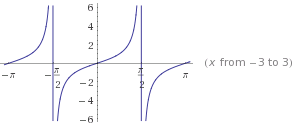
\includegraphics{1.png} 
      \end{minipage}
      \begin{itemize}
	\item $\diff{x}\tan x=\diff{x}\frac{\sin x}{\cos x}=\frac{\cos^2 x+\sin^2 x}{\cos^2 x}=1+\tan^2 x$
	\item $\diff{x}(1+\tan^2x)=2(1+\tan^2x)\tan x$
      \end{itemize}
    ~\item 
      \begin{minipage}{\linewidth}
	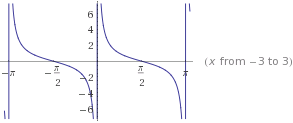
\includegraphics{2.png} 
      \end{minipage}
      \begin{itemize}
	\item $\diff{x}\cot x=\diff{x}\frac{\cos x}{\sin x}=\frac{-\sin^2(x)-\cos^2(x)}{sin^2 x}=-1-\cot^2 x$
	\item $\diff{x}(-1-\cot^2 x)=2(1+\cot^2 x)\cot x$
      \end{itemize}
    ~\item 
      \begin{minipage}{\linewidth}
	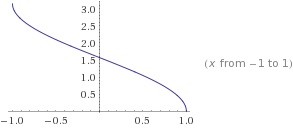
\includegraphics{3.png} 
      \end{minipage}
      \begin{itemize}
	\item $y=\arccos(x)\iff\cos y=x\implies\diff{x}\cos y=\diff{x}x\iff-\difff{y}{x}\sin y=1\iff -\difff{y}{x}\sqrt{1-\cos^2 y}=1\iff\difff{y}{x}=-\frac{1}{\sqrt{1-x^2}}$
	\item $\diff{x}-\frac{1}{\sqrt{1-x^2}}=-2x*\frac{-1}{2}(1-x^2)^{-3/2}=\frac{x}{\sqrt{(1-x^2)^3}}$
      \end{itemize}
    ~\item 
      \begin{minipage}{\linewidth}
	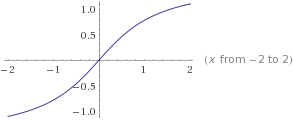
\includegraphics{4.png} 
      \end{minipage}
      \begin{itemize}
	\item $y=\arctan x\iff\tan y=x\implies\diff{x}\tan y=1\iff\difff{y}{x}(1+\tan^2y)=1\iff\difff{y}{x}=\frac{1}{1+x^2}$
	\item $\diff{x}\frac{1}{1+x^2}=-\frac{2x}{(1+x^2)^2}$
      \end{itemize}
    ~\item 
      \begin{minipage}{\linewidth}
	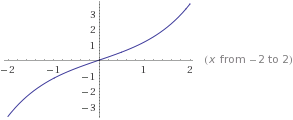
\includegraphics{5.png} 
      \end{minipage}
      \begin{itemize}
	\item $\diff{x}\sinh x=\diff{x}\frac{1}{2}(e^x-e^{-x})=\frac{1}{2}(e^x+e^-x)=\cosh x$
	\item $\diff{x}\cosh x=\diff{x}\frac{1}{2}(e^x+e^{-x})=\frac{1}{2}(e^x-e^{-x})=\sinh x$
	\item $\lim_{x\to\infty}\sinh x=\frac{1}{2}\lim_{x\to\infty}e^x=\infty$
	\item $\lim_{x\to-\infty}\sinh x=-\frac{1}{2}\lim_{x\to-\infty}e^{-x}=-\infty$
      \end{itemize}
    ~\item 
      \begin{minipage}{\linewidth}
	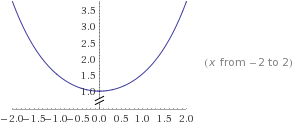
\includegraphics{6.png} 
      \end{minipage}
      \begin{itemize}
	\item Ableitungen siehe (5) 
	\item $\lim_{x\to\infty}\cosh x=\frac{1}{2}\lim_{x\to\infty}e^x=\infty$
	\item $\lim_{x\to-\infty}\cosh x=\frac{1}{2}\lim_{x\to\infty}e^x=\infty$
      \end{itemize}
    ~\item 
      \begin{minipage}{\linewidth}
	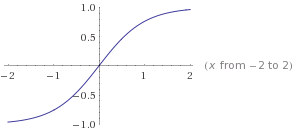
\includegraphics{7.png} 
      \end{minipage}
      \begin{itemize}
	\item $\diff{x}\frac{\sinh x}{\cosh x}=\frac{\cosh^2(x)-\sinh^2(x)}{\cosh^2 x}=1-\tanh^2 x$
	\item $\diff{x}(1-\tanh^2 x)=-2(1-\tanh^2 x)\tanh x$
	\item $\lim_{x\to\infty}\tanh x=\frac{\lim_{x\to\infty}\sinh x}{\lim_{x\to\infty}\cosh x}=1$
	\item $\lim_{x\to-\infty}\tanh x=\frac{\lim_{x\to-\infty}\sinh x}{\lim_{x\to-\infty}\cosh x}=-1$
      \end{itemize}
    ~\item 
      \begin{minipage}{\linewidth}
	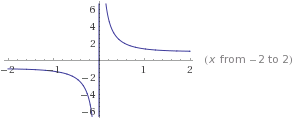
\includegraphics{8.png} 
      \end{minipage}
      \begin{itemize}
	\item $\diff{x}\frac{\cosh x}{\sinh x}=\frac{\sinh^2(x)-\cosh^2(x)}{\sinh^2 x}=1-\coth^2 x$
	\item $\diff{x}(1-\coth^2 x)=-2(1-\coth^2 x)\coth x$
	\item $\lim_{x\to\infty}\coth x=\frac{\lim_{x\to\infty}\cosh x}{\lim_{x\to\infty}\sinh x}=1$
	\item $\lim_{x\to-\infty}\coth x=\frac{\lim_{x\to-\infty}\cosh x}{\lim_{x\to-\infty}\sinh x}=-1$
      \end{itemize}
  \end{enumerate}
\stepcounter{aufgabe}
\end{aufgabe}
\begin{aufgabe}
  \begin{enumerate}
    ~\item $\abs{\vec{a}}=\sqrt{1^2+(-1)^2+2^2}=\sqrt{6}$ \\
      $\abs{\vec{b}}=\sqrt{4^2+3^2+0^2}=5$ \\
      $\abs{\vec{c}}=\sqrt{(-3)^2+3^2+(-6)^2}=\sqrt{54}=3\sqrt{6}$
    \item $\vec{a_n}=\frac{1}{\sqrt{6}}\vec{a}$ \\
      $\vec{b_n}=\frac{1}{5}\vec{b}$ \\
      $\vec{c_n}=\frac{1}{3\sqrt{6}}\vec{c}$
    \item
      \begin{itemize}
	\item $\vec{a}+\vec{b}=\colvec[5]{2}{2}$
	\item $\vec{a}+\vec{c}=\colvec[-2]{2}{-4}$
	\item $\vec{a}-\vec{b}=\colvec[-3]{-4}{2}$
	\item $\vec{a}-\vec{c}=\colvec[4]{-4}{8}$
	\item $\vec{a}*\vec{b}=1$
	\item $\vec{a}*\vec{c}=-18$
	\item $\vec{a}\times\vec{b}=\colvec[-6]{8}{7}$
	\item $\vec{a}\times\vec{c}=\colvec[0]{0}{0}=\vec{0}$
      \end{itemize}
    \item 
      \begin{itemize}
	\item $\vec{a}$ und $\vec{b}$: $\arccos(\frac{1}{\sqrt{6}*5})=\ang{85.32}$ 
	\item $\vec{a}$ und $\vec{c}$: $\arccos(\frac{-18}{\sqrt{6}*3*\sqrt{6}})=\pi$ 
      \end{itemize}
    \item $\frac{\vec{a}*\vec{b}}{\abs{\vec{b}}}=\frac{1}{5}$
  \end{enumerate}
\end{aufgabe}
\end{document}

